\chapter{Porównanie testowalności na przykładzie aplikacji}
\label{analiza_testow}

\section{Opis doświadczenia}
Doświadczenie polega na przeanalizowaniu przykładowej aplikacji dla Systemu Android zaprojektowanej na dwa sposoby. Wersja pierwsza to aplikacja napisana w standardowej architekturze (nazywana dalej \textit{wersją pierwotną}, wersja druga to ten sam program napisany przy wykorzystaniu \textit{Clean Architecture} (nazywana dalej \textit{wersją poprawioną}. Do tego celu zdecydowano się wykorzystać
aplikację \textit{JSON Web Token Authentication for Android} napisaną przez Victora Albertosa \cite{website:victor:aplication} , a której źródła udostępnione są w serwisie GitHub na licencji \textit{open source}.

W części doświadczalnej analizę ograniczono do analizy testowalności w zakresie testów jednostkowych i wczesnych testów integracyjnych pomijając analizę na etapie testów systemowych czy akceptacyjnych z powodu braku dostępu do wymagań systemowych i wymagań klienta. Jednakże już na podstawie analizy testów jednostkowych i wstępnego testu integracyjnego można z dużym prawdopodobieństwem ocenić, czy zastosowanie TDD i architektury \textit{Clean Architecture} poprawi testowalność programu i spowoduje ułatwienie dalszego procesu testowego.

\section{Opis aplikacji}
\textit{JSON Web Token Authentication for Android} autentykuje użytkowników Androida i iOS korzystając z \textit{REST API} serwera \textit{Parse} oraz textit{JSON\footnote{JSON, JavaScript Object Notation – lekki format wymiany danych komputerowych. JSON jest formatem tekstowym, bazującym na podzbiorze języka JavaScript. Źródło: Wikipedia.} Web Tokens (JWT)}. JWT to otwarta, według standardu przemysłowego RFC 7519\cite{website:jwt:rfc7519}, metoda do uwierzytelniania stron w środowisku aplikacji internetowych. Wykorzystywana jest do przekazywania tożsamości użytkowników między dostawcą, a odbiorcą usług internetowych lub innego typu uwierzytelnień zgodnie z logiką biznesową. 

Serwer \textit{Parse} to wspólna platforma do przechowywania danych i interakcji z usługami internetowymi dla aplikacji mobilnych. Wielu programistów decyduje się na wykorzystanie tej platformy, zamiast pisać własne rozwiązania w tym zakresie.

Victor Albertos zdecydował się użyć wyżej wymienionego rozwiązania, aby zwiększyć pielęgnowalność swojej aplikacji: móc modyfikować logikę biznesową nie modyfikując aplikacji po stronie klienta. Serwer Parse, jako rozwiązanie uniwersalne, zapewniał takie podejście i wpisywał się doskonale w koncepcję autora aplikacji.

\section{Zasada działania}
Użytkownik loguje się za pomocą swojej nazwy użytkownika i hasła do serwera \textit{Parse}. Jeżeli nie posiada jeszcze konta na serwerze, może założyć je bezpośrednio z używanego programu. Jeżeli użytkownik istnieje, od chwili zalogowania może korzystać z dostępnych mu usług serwera, a logując się z wielu urządzeń korzysta z wielosesyjności systemu. 

\section{Analiza aplikacji pod względem testowalności}
W tej pracy autor skupia się na budowie aplikacji tylko z punktu widzenia testowania aplikacji, nie będzie więc analizowany szczegółowo kod programu. Przeprowadzone natomiast zostaną testy, na podstawie których można w wystarczającej części ocenić, czy zmiana struktury oprogramowania na \textit{Clean Architecture} oraz zastosowanie  \textit{Test Driven Development} wpłynie pozytywnie na testowalność oprogramowania, w tym przypadku tej wybranej aplikacji.

\newpage
\subsection{Budowa analizowanej aplikacji w wersji pierwotnej}
Schemat budowy aplikacji \textit{JSON Web Token Authentication for Android} w wersji pierwotnej przedstawia się tak, jak to pokazano na rysunku \ref{fig:app_std}.

\begin{figure}[!htb]
    \centering
    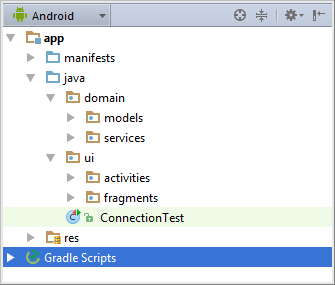
\includegraphics[width=8cm]{imgs/ch6_app_st.png}
    \caption
{Schemat budowy badanej aplikacji wykorzystującej architekturę standardową}
    \label{fig:app_std}
\end{figure} 

Aplikacja podzielona jest na moduł domeny i moduł interfejsu użytkownika. W celu przetestowania aplikacji, utworzono jeden test całkowicie zależny od środowiska Android, który w zależności od kontekstu można nazwać integracyjnym, systemowym, bądź nawet końcowym. Dla potrzeb pracy traktowany jest jako test integracyjny, gdyż interesuje autora tylko wynik weryfikacji połączenia, bez zwracania uwagi na aspekty graficzne czy użytkowe wiązane z docelowym urządzeniem. Test polega na zalogowaniu się do programu za pomocą przykładowych danych i otrzymaniu wyniku, czy weryfikacja przebiegła pomyślnie. Poza tym przypadkiem nie stwierdzono żadnych innych testów, w tym jednostkowych.

\subsection{Budowa analizowanej aplikacji w wersji poprawionej}
Każde z wymienionych w rozdziale \ref{propozycja_rozwiazania} podejść do uporządkowania architektury systemowej można wykorzystać do polepszenia testowalności aplikacji tworzonych dla systemu Android. Analizując opisywane rozwiązania krok po kroku można dojść do wniosku, że ich idea jest taka sama, a różnią się jedynie szczegółami. W tym wypadku autor \textit{JSON Web Token Authentication for Android} zdecydował się na \textit{The Clean Architecture}, zaprezentowaną w tej pracy w rozdziale \ref{clean_architecture_opis}.

Aplikacja w wersji poprawionej nadal ma budowę modułową - tym razem moduły są trzy: moduł domeny, moduł danych i moduł prezentacyjny. Zgodnie z nowym podejściem (patrz rysunek \ref{fig:clean_architecture} można rozpoznać poszczególne warstwy uporządkowanej architektury:
\begin{itemize}
\item
Warstwę \textit{entities}, w której znajduje się definicja klasy \textit{User} (rysunek ) oraz klasy \textit{Credentials}. Należą one do logiki biznesowej aplikacji i to na tych klasach oparte jest działanie programu. 
\begin{figure}[!htb]
    \centering
    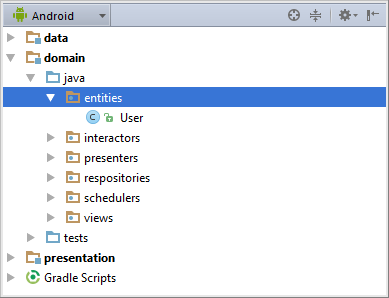
\includegraphics[width=8cm]{imgs/ch6_app_cl_entities.png}
    \caption
{Schemat budowy aplikacji w wersji poprawionej: warstwa \textit{entities}}
    \label{fig:app_cl_entities}
\end{figure} 

\item
Warstwę \textit{Use Cases}, należącą do modułu domeny, do której na podstawie przypadków użycia zostały napisane testy jednostkowe (patrz rysunek \ref{fig:app_cl_usecases})
\begin{figure}[!htb]
    \centering
    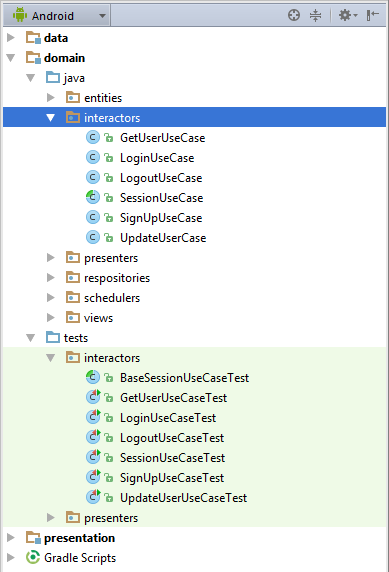
\includegraphics[width=8cm]{imgs/ch6_app_cl_usecases.png}
    \caption
{Schemat budowy aplikacji w wersji poprawionej: warstwa \textit{use cases}}
    \label{fig:app_cl_usecases}
\end{figure} 

\item
Warstwę \textit{Presenters}, również należącą do modułu domenowego i odpowiadające jej testy jednostkowe (rysunek \ref{fig:app_cl_presenters}).
\begin{figure}[!htb]
    \centering
    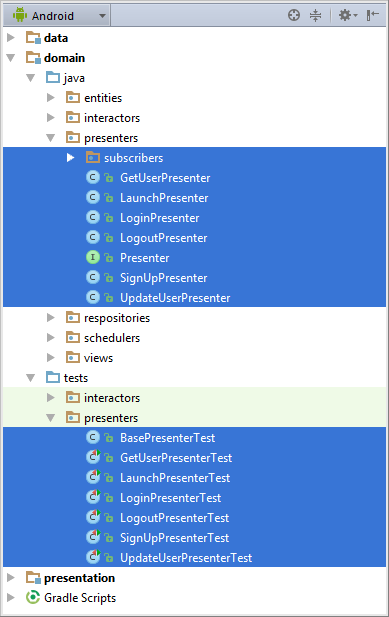
\includegraphics[width=8cm]{imgs/ch6_app_cl_presenters.png}
    \caption
{Schemat budowy aplikacji w wersji poprawionej: warstwa \textit{presenters}}
    \label{fig:app_cl_presenters}
\end{figure} 

\item
Moduły \textit{data} oraz \textit{presentation}, to najbardziej zewnętrzna warstwa, zależna od wszystkich wyżej opisanych. 
\end{itemize}

Zgodnie z ideą uporządkowanej architektury, warstwa \textit{entities} nie ma danych na temat warstwy \textit{use cases}, przypadki użytkownika nie wiedzą nic o warstwie prezentacyjnej, a ta nie posiada informacji o warstwach zewnętrznych, takich jak wspomniane bazy danych. Kierunek wstrzykiwania zależności jest zawsze od warstwy zewnętrznej do warstwy wewnętrznej, co pokazuje rysunek \textbf{narysować zalezności}.

\textit{tutaj rysunek zależności}

\section{Przebieg doświadczenia}
Podczas doświadczenia wykonany dostępne testy dla obu wersji programu, wykorzystując to samo środowisko testowe (\textit{wziąć pojęcia ze słownika testerskiego}): Android Studio w wersji 1.5.1, ten sam komputer i ten sam emulator: Nexus\_5\_API\_23. Przeprowadzono również analizę wyników.

\section{Wyniki doświadczenia}
\label{wyniki_doswiadczenia}
\subsection{Testy jednostkowe}
Wyniki doświadczenia dla testów jednostkowych przedstawiają się następująco:
W przypadku aplikacji w wersji poprawionej testy jednostkowe istnieją dla warstw \textit{use cases} oraz \textit{presenters} Rezultat wykonania przedstawiają tabele \ref{fig:app_cl_test5}, \ref{fig:app_cl_test3} i \ref{fig:app_cl_test4}.

\begin{figure}[!htb]
    \centering
    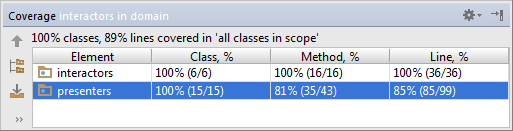
\includegraphics[width=12cm]{imgs/ch6_app_cl_test5.png}
    \caption
{Wyniki wraz z pokryciem kodu}
    \label{fig:app_cl_test5}
\end{figure} 

\begin{figure}[!htb]
    \centering
    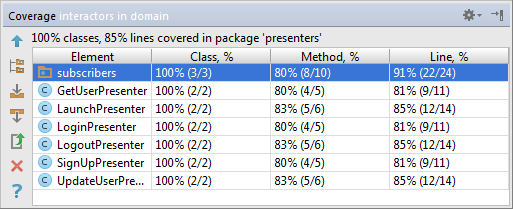
\includegraphics[width=12cm]{imgs/ch6_app_cl_test3.png}
    \caption
{Wyniki wraz z pokryciem kodu}
    \label{fig:app_cl_test3}
\end{figure} 

\begin{figure}[!htb]
    \centering
    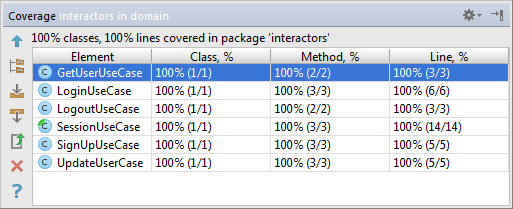
\includegraphics[width=12cm]{imgs/ch6_app_cl_test4.png}
    \caption
{Wyniki wraz z pokryciem kodu}
    \label{fig:app_cl_test4}
\end{figure} 

W aplikacji w wersji pierwotnej testów jednostkowych nie zaprojektowano w ogóle, a testując funkcjonalność programu zdano się w całości na automatyczny test integracyjny. 

W przypadku aplikacji w wersji poprawionej, jak przedstawiają tabele aaaaaaa i bbbbbbb, zaprojektowano 6 testów opartych na przypadkach użycia oraz 7 testów dla prezenterów, co daje łącznie 13 testów jednostkowych. W przypadku aplikacji w wersji pierwszej - zgodnie z wyjaśnieniem, które autor umieścił w rozdziale \ref{testowanie_starej_struktury} - aby pokryć ten sam obszar funkcjonalności należałoby zaprojektować 6 * 7 = 42 testy jednostkowe.

\textit{rysunek pierwszy - różnice w ilości testów jednostkowych dla obu aplikacji}

Taka liczba testów musiała się również odbić na ich czasie wykonania, co w przypadku badanej aplikacji przedstawia się następująco:

\textit{rysunek drugi - różnice w czasie wykonania testów jednostkowych dla obu aplikacji}
 
\subsection{Testy integracyjne}
Jak już wspomniano wcześniej, w przypadkach obu wersji oprogramowania zaprojektowano test integracyjny \textit{ConnectionTest}. Zakres testu taki sam dla obu opisywanych przypadków: generowany jest zestaw kilku użytkowników dla których przeprowadzana jest próba połączenia. Czas trwania całego testu od uruchomienia do otrzymania wyniku pozytywnego bądź negatywnego (wraz z uruchomieniem emulatora systemu Android) wyliczony w doświadczeniu wyniósł około 200 sekund. 

W przypadku gdy dla aplikacji w wersji pierwszej nie stwierdzono testów jednostkowych, to
\begin{itemize}
\item
zakładając, że każdy z sześciu testów jednostkowych opartych na przypadkach użycia dla aplikacji w wersji poprawionej znalazłby jeden błąd, liczba powtórzeń testu \textit{ConnectionTest} w najgorszym razie mogłaby wzrosnąć sześciokrotnie;
\item
zakładając, że dodatkowo każdy z siedmiu testów jednostkowych przeznaczonych dla prezenterów również znalazłby błąd, ilość powtórzeń testu \textit{ConnectionTest} w najgorszym przypadku mogłaby wzrosnąć 42-krotnie do momentu uzyskania wyniku pozytywnego.

\textit{wykresik ładny w excelu zrobić}
\end{itemize}

\begin{figure}[!htb]
    \centering
    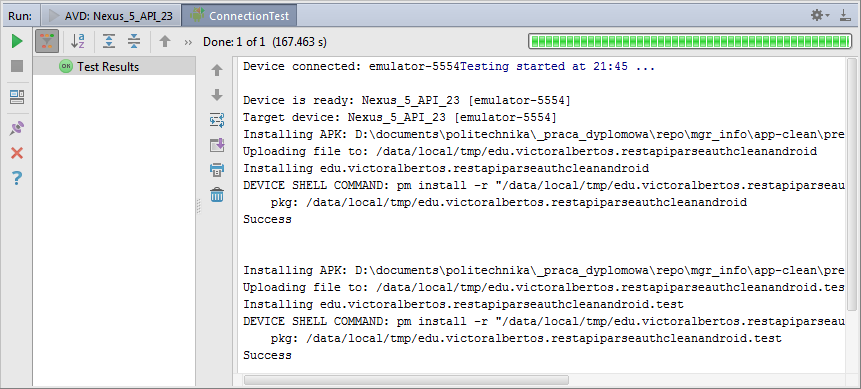
\includegraphics[width=15cm]{imgs/ch6_app_cl_test6.png}
    \caption
{Wynik testu integracyjnego}
    \label{fig:app_cl_test6}
\end{figure} 

\section{Wnioski końcowe}
Wykorzystanie \textit{Clean Architecture} wydaje się właściwe dla polepszenia testowalności badanej aplikacji zarówno w przypadku, gdy posiadałaby ona testy jednostkowe (patrz rysunek .....), jak również w sytuacji badanej, kiedy testów jednostkowych nie napisano w ogóle, jak w zastanej sytuacji (rysunek ......).

Nawet jeżeli testy jednostkowe zostałyby napisane, do przetestowania tego samego obszaru funkcjonalności ich liczba musiałaby być zdecydowanie większa od liczby ich odpowiedników w przypadku aplikacji poprawionej, co wymaga odpowiednio większego nakładu pracy pielęgnacyjnej w przypadku przeprowadzania modyfikacji programu. Zmiana kodu programu w przypadku rozszerzenia funkcjonalności również wymagałaby napisania większej ilości dodatkowych testów jednostkowych.

Gdy testów jednostkowych, tak jak w badanym przypadku, nie ma, wtedy potrzeba zwiększenia czasu przeznaczonego na testy integracyjne i wyższego szczebla jest jeszcze większa. 

Wynik doświadczenia pokazuje jasno, że warto wykorzystać opisywane w rozdziale \ref{propozycja_rozwiązania} metody do zwiększenia testowalności i także, jak się okazuje, pielęgnowalności aplikacji przeznaczonych dla systemu Android. 